\documentclass[conference]{IEEEtran}
% \IEEEoverridecommandlockouts
% The preceding line is only needed to identify funding in the first footnote. If that is unneeded, please comment it out.
%Template version as of 6/27/2024

\usepackage{cite}
\usepackage{amsmath,amssymb,amsfonts}
\usepackage{algorithmic}
\usepackage{graphicx}
\usepackage{textcomp}
\usepackage{xcolor}
\usepackage{fancyhdr}
\usepackage[skip=3.3pt, indent=5mm]{parskip}

\def\BibTeX{{\rm B\kern-.05em{\sc i\kern-.025em b}\kern-.08em
    T\kern-.1667em\lower.7em\hbox{E}\kern-.125emX}}
\begin{document}

\title{Hållbarhetsrapport\\
% {\footnotesize \textsuperscript{*}Note: Sub-titles are not captured for https://ieeexplore.ieee.org  and
% should not be used}
% \thanks{Identify applicable funding agency here. If none, delete this.}
}

\author{\IEEEauthorblockN{Erik Forsberg}
\IEEEauthorblockA{\textit{Högskoleingenjörsprogrammet inom Datateknik} \\
\textit{KTH}\\
Stockholm, Sverige \\
erforsbe@kth.se}
}

\maketitle

% Adds page numbers
\thispagestyle{plain}
\pagestyle{plain}

\begin{abstract}
Denna rapport studerar artificiell intelligens ur ett hållbarhetsperspektiv. Fördelar och nackdelar av konstruktion, underhåll och användning observeras följt av några lösningsförslag.
Miljöpåverkan av artificiell intelligens är svårdefinierad av flera anledningar, men det är tydligt att teknologin har både positiva och negativa implikationer för hälsan av vår planet.
\end{abstract}

\begin{IEEEkeywords}
hållbarhet, miljö, teknik, artificiell intelligens, fördelar, nackdelar
\end{IEEEkeywords}

\section{Introduktion}

Sedan artificiell intelligens (AI) för några är sedan hade sina största genombrott så har teknologins utveckling och användning ökat i hisnande hastighet. Det nästlar in sig i fler och fler aspekter av vår dagliga teknologianvändning \cite{b1} och tack vare att enorma mängder pengar investeras i teknologin så projiceras den att fortsätta växa snabbt inom de kommande åren \cite{b2}. 

Det är även en teknologi som påverkar många människors arbeten och hur de utförs och i många fall uppstår oro över huruvida man riskerar att förlora sitt jobb till en AI-modell som kan utföra arbetet snabbare \cite{b3}. 

Med ovanstående i åtanke är det föga förvånande att ämnet dominerar stora delar av teknologisk diskussion. Den om AI är en diskussion som präglas av starka åsikter där det talas om allt från utopisk optimism till apokalyptisk pessimism, men oavsett var en själv står kan det vara svårt att bortse från potentialen för både positiva och negativa utfall för alla nivåer av samhället. 

En ofta underrepresenterad diskussionspunkt är dock AI:s påverkan på vår miljö. Det är en nyanserad fråga som beroende på ståndpunkt kan ha helt olika svar och kan därför inte besvaras med en tydlig slutsats. Den här rapporten kommer att presentera de olika synvinklarna och lämna vidare övervägande till läsaren. 

\section{Utopi - Vad AI kan göra för en hållbar framtid}

Användning av AI har stort potential att hjälpa människor utföra uppgifter som är tidskrävande och/eller svåra för människor. Hantering av stora mängder data \cite{b4} och övermänsklig mönsterigenkänning \cite{b5} är sådant som kan användas i syfte att förbättra, optimera och analysera olika processer ur miljösynpunkt.  

Detta har prövats med goda resultat i till exempel kemiindustrin redan 2021 då de fann stor potential för förminskning av energikonsumtion, miljöpåverkan och risker vid kemisk produktion \cite{b6}.

Hos aktuella användningsfall av AI i miljösyfte finner vi bland annat Förenta nationernas miljöprogram. Där använder de sig av AI för att analysera stora mängder data om metanutsläpp och kompilerar den datan i olika format vilket underlättar för vidare analys och forskning om ämnet \cite{b7}. Vi finner även Google, en av de ledande aktörerna inom teknologin, som använder sig av AI för att optimera deras vägledningsalgoritmer i syfte att reducera utsläpp genom att föreslå bränslesnålare vägar samt genom att dirigera trafiken på ett bränsleeffektivt vis genom uppkopplade trafikljus \cite{b8}. 

\section{Dystopi - AI:s påfrestningar på miljön}

Miljökostnaderna för de fysiska systemen bakom AI är stora vid alla punkter av dess livstider. AI drivs huvudsakligen från stora datacenter där den höga utvecklingstakten innebär att ny hårdvara installeras med korta mellanrum vilket leder till att den gamla hårdvaran kastas, ofta utan att återvinnas \cite{b9}.

Under dess livslängd så kommer de komponenter som driver AI också att dra stora mängder energi vilket leder till stora mängder värme som i sin tur måste kylas ner. Den nedkylningen sker främst genom vattenkylning, en process som kan kräva flera miljoner liter vatten enbart för att träna en enda AI-modell \cite{b10}. 

Utöver dessa fysiska kostnader så presenteras risker i hur människor använder AI. Som konsekvens av att generativ AI är föga mer än en matematisk modell snarare än ett resonerande intellekt så följer en hög risk för generering av falsk information \cite{b11}. Denna falska information kan spridas snabbt, bland annat genom vetenskapliga skrifter vars författare brukat generativ AI vid skrivning \cite{b12}.  

AI gör det också lättare att generera material som själviska aktörer kan använda för att sprida falsk information om miljöfrågor \cite{b13}. I en värld där fossilindustrin och deras associerade organisationer spenderar pengar på att sakta ner miljöpositiv lagstiftning \cite{b14} och sprida falsk information om miljön på sociala medier \cite{b15} så är generativ AI ytterligare ett vapen i deras arsenal. 

\section{Lösningar - Vad kan vi göra?}

Som konstaterat så är en stor andel av AI:s miljöpåverkan en konsekvens av konstruktionen och underhållningen av datacenter. Ansvar för att detta sker på ett miljövänligt sätt ligger därmed hos de företag som driver verksamheten, men även på lagstiftningen av de länder som verksamheten äger rum i. Ett exempel på lagliga åtgärder som godkänts är EU:s “Artifical Intelligence Act” som bland annat ämnar minska AI:s miljöpåverkan \cite{b16}.  

Även individen kan göra sitt för att agera miljömedvetet vid användning av AI. Olika sorters prompts ställda till olika sorters generativa AI-chattbottar drar olika mängder energi \cite{b17} vilket innebär att det finns bättre och sämre sätt att bruka AI ur miljöperspektiv. Huggingface driver ett “Energy score leaderboard” på sin hemsida \cite{b18} där man kan jämföra olika modellers effektivitet när de utför olika uppgifter. Se bilaga 1 för en visualisering av hur mycket energi de olika uppgifterna kräver \cite{b19}. 

\section{Dilemmat - en sorts slutsats}
AI utvecklas fortfarande vilket gör det svårt att göra en konkret bedömning om huruvida den miljöpåverkan AI ger upphov till är värt produkten. Vi har ej ännu hittat gränsen av denna teknologi, om en sådan finns, vilket innebär att AI en dag kan vara det som ger oss lösningen till de miljöproblem som det idag ger upphov till. Om en sådan dag kommer så kan man argumentera att miljökostnaden är rättfärdigad, men tills dess så är det klokaste kanske att observera AI för hur det i dagsläget ser ut och hitta lösningar som förbättrar läget i stunden. 

\begin{thebibliography}{00}
\bibitem{b1}N. Maslej, L. Fattorini, R. Perrault, Y. Gil, V. Parli, N. Kariuki, et al. “The AI Index 2025 Annual Report,” Stanford, Apr. 2025. https://hai.stanford.edu/ai-index/2025-ai-index-report (hämtad Sep. 09, 2025). 
\bibitem{b2}UNCTAD, “AI Market Projected to Hit \$4.8 Trillion by 2033, Emerging as Dominant Frontier Technology,” UN Trade and Development (UNCTAD), Apr. 07, 2025. https://unctad.org/news/ai-market-projected-hit-48-trillion-2033-emerging-dominant-frontier-technology (hämtad Sep. 09, 2025). 
\bibitem{b3}C. Pazzanese, “Will your job survive AI?,” Harvard Gazette, Jul. 29, 2025. https://news.harvard.edu/gazette/story/2025/07/will-your-job-survive-ai/ (hämtad Sep. 09, 2025). 
\bibitem{b4}“What is big data? | Big data and AI,” Cloudflare.com, 2024. https://www.cloudflare.com/learning/ai/big-data/ (hämtad Sep. 09, 2025). 
\bibitem{b5}P. Bansal, “AI Pattern Recognition and its Features,” International Journal of Engineering and Advanced Technology, vol. 14, no. 3, pp. 1, Feb. 2025. https://www.researchgate.net/publication/389173710\_AI
\_Pattern\_Recognition\_and\_its\_Features (hämtad Sep. 09, 2025). 
\bibitem{b6}M. Liao, K. Lan, and Y. Yao, “Sustainability implications of artificial intelligence in the chemical industry: A conceptual framework,” Journal of Industrial Ecology, vol. 26, no. 1, Nov. 2021. https://onlinelibrary.wiley.com/doi/full/10.1111/jiec.13214 (hämtad Sep. 09, 2025). 
\bibitem{b7}"Eye on Methane data platform | IMEO,” Eye on Methane, 2024. https://methanedata.unep.org/ (hämtad Sep. 09, 2025). 
\bibitem{b8}“Google AI - Sustainability AI,” Ai.google, 2021. https://ai.google/sustainability/ (hämtad Sep. 09, 2025). 
\bibitem{b9}C. Crownhart, “AI will add to the e-waste problem. Here’s what we can do about it.,” MIT Technology Review, Oct. 28, 2024. https://www.technologyreview.com/2024/10/28/1106316/ai-e-waste/ (hämtad Sep. 09, 2025). 
\bibitem{b10}P. Li, J. Yang, M. Islam, and S. Ren, “Making AI Less ‘Thirsty’: Uncovering and Addressing the Secret Water Footprint of AI Models,” Mar. 2025. https://arxiv.org/pdf/2304.03271 (hämtad Sep. 09, 2025). 
\bibitem{b11}C. for C. D. Hate, “The Double-Edged Sword of AI: How Generative Language Models Like Google Bard and ChatGPT Pose a Threat to Countering Hate and Misinformation Online,” Harvard Data Science Review, no. Special Issue 5, Dec. 2024. https://hdsr.mitpress.mit.edu/pub/vn2v6ety/release/1 (hämtad Sep. 09, 2025). 
\bibitem{b12}J. Haider, Kristofer Rolf Söderström, Björn Ekström, and Malte Rödl, “GPT-fabricated scientific papers on Google Scholar: Key features, spread, and implications for preempting evidence manipulation,” Sep. 2024. https://misinforeview.hks.harvard.edu/article/gpt-fabricated-scientific-papers-on-google-scholar-key-features-spread-and-implications-for-preempting-evidence-manipulation/ (hämtad Sep. 09, 2025). 
\bibitem{b13}V. Galaz, S. Daume, and Arvid Marklund, “A game changer for misinformation: The rise of generative AI,” stockholmresilience.org, May 25, 2023. https://www.stockholmresilience.org/news--events/climate-misinformation/chapter-6-a-game-changer-for-misinformation-the-rise-of-generative-ai.html (hämtad Sep. 12, 2025). 
\bibitem{b14}R. Sullivan, R. Black, and G. Kyriacou, “What is climate change lobbying?” Grantham Research Institute on climate change and the environment, Feb. 17, 2023. https://www.lse.ac.uk/granthaminstitute/explainers/what-is-climate-change-lobbying/ (hämtad Sep. 09, 2025). 
\bibitem{b15}J. Turrentine, “Climate Misinformation on Social Media Is Undermining Climate Action,” NRDC, Apr. 19, 2022. https://www.nrdc.org/stories/climate-misinformation-social-media-undermining-climate-action (hämtad Sep. 09, 2025). 
\bibitem{b16}“Texts adopted - Artificial Intelligence Act - Wednesday, 13 March 2024,” www.europarl.europa.eu, Mar. 13, 2024. https://www.europarl.europa.eu/doceo/document/TA-9-2024-0138\_EN.html (hämtad Sep. 09, 2025). 
\bibitem{b17}K. Griesser, “Study reveals how much energy AI uses to answer your questions,” CNN, Jun. 22, 2025. https://edition.cnn.com/2025/06/22/climate/ai-prompt-carbon-emissions-environment-wellness (hämtad Sep. 09, 2025). 
\bibitem{b18}“AI Energy Score Leaderboard,” Huggingface.co, 2025. https://huggingface.co/spaces/AIEnergyScore/Leaderboard (hämtad Sep. 09, 2025). 
\bibitem{b19}S. Chen, “How much energy will AI really consume? The good, the bad and the unknown,” Nature, vol. 639, no. 8053, pp. 22–24, Mar. 2025. https://www.nature.com/articles/d41586-025-00616-z (hämtad Sep. 09, 2025).
\end{thebibliography}

\cleardoublepage
\onecolumn
\section*{Bilagor}
\vspace{8ex}
\centerline{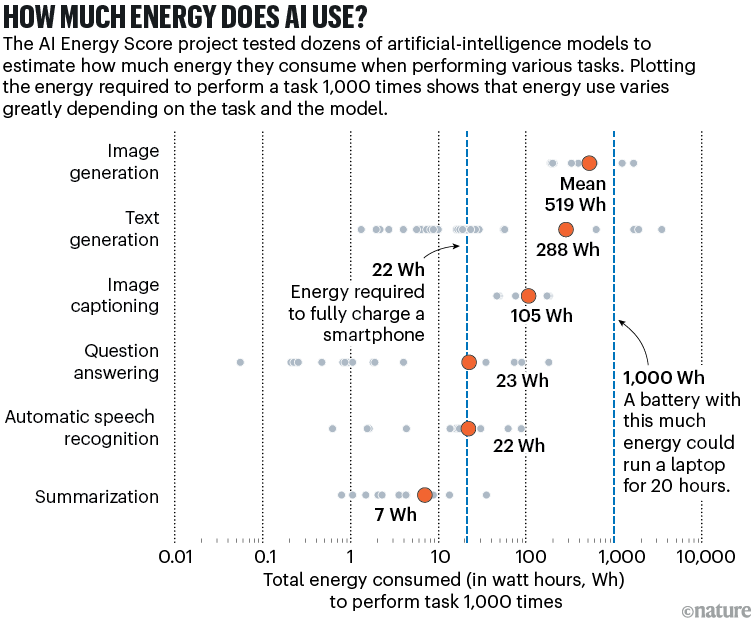
\includegraphics[width=0.8\textwidth]{bilaga1.png}}
\centerline{Bilaga 1. Diagram som illustrerar olika AI-uppgifters energikonsumtion.}

\end{document}
